\documentclass[]{article}
\usepackage{lmodern}
\usepackage{amssymb,amsmath}
\usepackage{ifxetex,ifluatex}
\usepackage{fixltx2e} % provides \textsubscript
\ifnum 0\ifxetex 1\fi\ifluatex 1\fi=0 % if pdftex
  \usepackage[T1]{fontenc}
  \usepackage[utf8]{inputenc}
\else % if luatex or xelatex
  \ifxetex
    \usepackage{mathspec}
  \else
    \usepackage{fontspec}
  \fi
  \defaultfontfeatures{Ligatures=TeX,Scale=MatchLowercase}
\fi
% use upquote if available, for straight quotes in verbatim environments
\IfFileExists{upquote.sty}{\usepackage{upquote}}{}
% use microtype if available
\IfFileExists{microtype.sty}{%
\usepackage{microtype}
\UseMicrotypeSet[protrusion]{basicmath} % disable protrusion for tt fonts
}{}
\usepackage[margin=1in]{geometry}
\usepackage{hyperref}
\hypersetup{unicode=true,
            pdfborder={0 0 0},
            breaklinks=true}
\urlstyle{same}  % don't use monospace font for urls
\usepackage{color}
\usepackage{fancyvrb}
\newcommand{\VerbBar}{|}
\newcommand{\VERB}{\Verb[commandchars=\\\{\}]}
\DefineVerbatimEnvironment{Highlighting}{Verbatim}{commandchars=\\\{\}}
% Add ',fontsize=\small' for more characters per line
\usepackage{framed}
\definecolor{shadecolor}{RGB}{248,248,248}
\newenvironment{Shaded}{\begin{snugshade}}{\end{snugshade}}
\newcommand{\KeywordTok}[1]{\textcolor[rgb]{0.13,0.29,0.53}{\textbf{#1}}}
\newcommand{\DataTypeTok}[1]{\textcolor[rgb]{0.13,0.29,0.53}{#1}}
\newcommand{\DecValTok}[1]{\textcolor[rgb]{0.00,0.00,0.81}{#1}}
\newcommand{\BaseNTok}[1]{\textcolor[rgb]{0.00,0.00,0.81}{#1}}
\newcommand{\FloatTok}[1]{\textcolor[rgb]{0.00,0.00,0.81}{#1}}
\newcommand{\ConstantTok}[1]{\textcolor[rgb]{0.00,0.00,0.00}{#1}}
\newcommand{\CharTok}[1]{\textcolor[rgb]{0.31,0.60,0.02}{#1}}
\newcommand{\SpecialCharTok}[1]{\textcolor[rgb]{0.00,0.00,0.00}{#1}}
\newcommand{\StringTok}[1]{\textcolor[rgb]{0.31,0.60,0.02}{#1}}
\newcommand{\VerbatimStringTok}[1]{\textcolor[rgb]{0.31,0.60,0.02}{#1}}
\newcommand{\SpecialStringTok}[1]{\textcolor[rgb]{0.31,0.60,0.02}{#1}}
\newcommand{\ImportTok}[1]{#1}
\newcommand{\CommentTok}[1]{\textcolor[rgb]{0.56,0.35,0.01}{\textit{#1}}}
\newcommand{\DocumentationTok}[1]{\textcolor[rgb]{0.56,0.35,0.01}{\textbf{\textit{#1}}}}
\newcommand{\AnnotationTok}[1]{\textcolor[rgb]{0.56,0.35,0.01}{\textbf{\textit{#1}}}}
\newcommand{\CommentVarTok}[1]{\textcolor[rgb]{0.56,0.35,0.01}{\textbf{\textit{#1}}}}
\newcommand{\OtherTok}[1]{\textcolor[rgb]{0.56,0.35,0.01}{#1}}
\newcommand{\FunctionTok}[1]{\textcolor[rgb]{0.00,0.00,0.00}{#1}}
\newcommand{\VariableTok}[1]{\textcolor[rgb]{0.00,0.00,0.00}{#1}}
\newcommand{\ControlFlowTok}[1]{\textcolor[rgb]{0.13,0.29,0.53}{\textbf{#1}}}
\newcommand{\OperatorTok}[1]{\textcolor[rgb]{0.81,0.36,0.00}{\textbf{#1}}}
\newcommand{\BuiltInTok}[1]{#1}
\newcommand{\ExtensionTok}[1]{#1}
\newcommand{\PreprocessorTok}[1]{\textcolor[rgb]{0.56,0.35,0.01}{\textit{#1}}}
\newcommand{\AttributeTok}[1]{\textcolor[rgb]{0.77,0.63,0.00}{#1}}
\newcommand{\RegionMarkerTok}[1]{#1}
\newcommand{\InformationTok}[1]{\textcolor[rgb]{0.56,0.35,0.01}{\textbf{\textit{#1}}}}
\newcommand{\WarningTok}[1]{\textcolor[rgb]{0.56,0.35,0.01}{\textbf{\textit{#1}}}}
\newcommand{\AlertTok}[1]{\textcolor[rgb]{0.94,0.16,0.16}{#1}}
\newcommand{\ErrorTok}[1]{\textcolor[rgb]{0.64,0.00,0.00}{\textbf{#1}}}
\newcommand{\NormalTok}[1]{#1}
\usepackage{longtable,booktabs}
\usepackage{graphicx,grffile}
\makeatletter
\def\maxwidth{\ifdim\Gin@nat@width>\linewidth\linewidth\else\Gin@nat@width\fi}
\def\maxheight{\ifdim\Gin@nat@height>\textheight\textheight\else\Gin@nat@height\fi}
\makeatother
% Scale images if necessary, so that they will not overflow the page
% margins by default, and it is still possible to overwrite the defaults
% using explicit options in \includegraphics[width, height, ...]{}
\setkeys{Gin}{width=\maxwidth,height=\maxheight,keepaspectratio}
\IfFileExists{parskip.sty}{%
\usepackage{parskip}
}{% else
\setlength{\parindent}{0pt}
\setlength{\parskip}{6pt plus 2pt minus 1pt}
}
\setlength{\emergencystretch}{3em}  % prevent overfull lines
\providecommand{\tightlist}{%
  \setlength{\itemsep}{0pt}\setlength{\parskip}{0pt}}
\setcounter{secnumdepth}{0}
% Redefines (sub)paragraphs to behave more like sections
\ifx\paragraph\undefined\else
\let\oldparagraph\paragraph
\renewcommand{\paragraph}[1]{\oldparagraph{#1}\mbox{}}
\fi
\ifx\subparagraph\undefined\else
\let\oldsubparagraph\subparagraph
\renewcommand{\subparagraph}[1]{\oldsubparagraph{#1}\mbox{}}
\fi

%%% Use protect on footnotes to avoid problems with footnotes in titles
\let\rmarkdownfootnote\footnote%
\def\footnote{\protect\rmarkdownfootnote}

%%% Change title format to be more compact
\usepackage{titling}

% Create subtitle command for use in maketitle
\newcommand{\subtitle}[1]{
  \posttitle{
    \begin{center}\large#1\end{center}
    }
}

\setlength{\droptitle}{-2em}

  \title{}
    \pretitle{\vspace{\droptitle}}
  \posttitle{}
    \author{}
    \preauthor{}\postauthor{}
    \date{}
    \predate{}\postdate{}
  

\begin{document}

Alyssa Vanderbeek (amv2187)\\
12 October 2018\\
HW 3

\subsubsection{Problem 1}\label{problem-1}

\subsubsection{1. Derive E(S2)}\label{derive-es2}

Let \(X_1, X_2, ..., X_n\) come from a distribution with mean \(\mu\)
and variance \(\sigma^2\). Let
\(S^2 = \frac{1}{n-1}\sum_{i=1}^n (X_i-\bar{X})^2\). Then

\[
\begin{aligned}
E(S^2) &= E[\frac{1}{n-1}\sum_{i=1}^n (X_i-\bar{X})^2] \\
&= \frac{1}{n-1}E[\sum_{i=1}^n (X_i-\bar{X})^2] \\
&= \frac{1}{n-1}E[\sum_{i=1}^n (X_i^2 - 2\bar{X}X_i^2-\bar{X}^2)] \\
&= \frac{1}{n-1}E[\sum_{i=1}^n X_i^2 - 2\bar{X} \sum_{i=1}^n X_i^2 - \sum_{i=1}^n \bar{X}^2)] \\
\end{aligned}
\]

Recall that
\(\bar{X} = \frac{\sum_{i=1}^n X_i}{n} \implies \sum_{i=1}^n X_i = n\bar{X}\).

\[
\begin{aligned}
&= \frac{1}{n-1}E[\sum_{i=1}^n X_i^2 - 2n\bar{X}^2 - n\bar{X}^2)] \\
&= \frac{1}{n-1}E[\sum_{i=1}^n X_i^2 - n\bar{X}^2)] \\
&= \frac{1}{n-1}[E(\sum_{i=1}^n X_i^2) - nE(\bar{X}^2)] \\
&= \frac{1}{n-1}[\sum_{i=1}^n E(X_i^2) - nE(\bar{X}^2)]
\end{aligned}
\]

Here we can make use of the identity \(Var(X) = E(X^2) - E(X)^2\), which
gives us \(E(X^2) = Var(X) + E(X) = \sigma^2 + \mu\) for all
\(X_i, i=1,2,..,n\). Additionally, note that for \(\bar{X}\), we have

\[
\begin{aligned}
Var(\bar{X}) &= Var(\frac{\sum_{i=1}^n X_i}{n}) \\
&= \frac{1}{n^2} Var(\sum_{i=1}^n X_i) \\
&= \frac{1}{n^2} \sum_{i=1}^n Var(X_i) \\
&= \frac{1}{n^2} \sum_{i=1}^n \sigma^2 \\
&= \frac{\sigma^2}{n} \\
\\
E(\bar{X}) &= E(\bar{X})^2 + Var(\bar{X}) \\
&= \mu^2 + \frac{\sigma^2}{n}
\end{aligned}
\]

Using these identities, we get

\[
\begin{aligned}
&= \frac{1}{n-1}[nE(X_i^2) - nE(\bar{X}^2)] \\
&= \frac{1}{n-1}[n (\mu^2 + \sigma^2) - n (\mu^2 + \frac{\sigma^2}{n})] \\
&= \frac{1}{n-1} (n\sigma^2 - \sigma^2) \\
&= \sigma^2
\end{aligned}
\]

Therefore, \(E(S^2) = \sigma^2\), showing that
\(S^2 = \frac{1}{n-1}\sum_{i=1}^n (X_i-\bar{X})^2\) is an unbiased
estimator of the true variance.

\subsubsection{2. Show that SS\_total = SS\_within +
SS\_between.}\label{show-that-ss_total-ss_within-ss_between.}

For \(k\) groups, each with \(n_i, i=1,2,...,k\) observations,

\[
\begin{aligned}
\sum_{i=1}^k \sum_{j=1}^{n_i} (Y_{ij} - \bar{Y})^2 &= 
  \sum_{i=1}^k \sum_{j=1}^{n_i} (Y_{ij} - \bar{Y}_i + \bar{Y}_i - \bar{Y})^2, \text{ where } \bar{Y}_i \text{ is the within-group average.}  \\
&= \sum_{i=1}^k \sum_{j=1}^{n_i} [ (Y_{ij} - \bar{Y}_i) + (\bar{Y}_i - \bar{Y}) ]^2 \\
&= \sum_{i=1}^k \sum_{j=1}^{n_i} [ (Y_{ij} - \bar{Y}_i)^2 + 2(Y_{ij} - \bar{Y}_i)(\bar{Y}_i - \bar{Y}) + (\bar{Y}_i - \bar{Y})^2 ] \\
&= \sum_{i=1}^k \sum_{j=1}^{n_i} (Y_{ij} - \bar{Y}_i)^2 + 2\sum_{i=1}^k \sum_{j=1}^{n_i}(Y_{ij} - \bar{Y}_i)(\bar{Y}_i - \bar{Y}) + \sum_{i=1}^k \sum_{j=1}^{n_i}(\bar{Y}_i - \bar{Y})^2 \\
\end{aligned}
\]

where
\(2\sum_{i=1}^k \sum_{j=1}^{n_i}(Y_{ij} - \bar{Y}_i)(\bar{Y}_i - \bar{Y}) = 2 \sum_{j=1}^{n_i}(Y_{ij} - \bar{Y}_i) \sum_{i=1}^k(\bar{Y}_i - \bar{Y}) = 0\),
since both \((Y_{ij} - \bar{Y}_i)\) and \((\bar{Y}_i - \bar{Y})\) are
residual terms, and the sum of residuals must be zero. Therefore, we are
left with

\[ 
\sum_{i=1}^k \sum_{j=1}^{n_i} (Y_{ij} - \bar{Y})^2 = \sum_{i=1}^k \sum_{j=1}^{n_i} (Y_{ij} - \bar{Y}_i)^2 + \sum_{i=1}^k \sum_{j=1}^{n_i}(\bar{Y}_i - \bar{Y})^2
\]

which states that the total variability (sum of squares) is equal to the
sum of the variability within groups and between groups.

\newpage

\subsubsection{\texorpdfstring{Problem 2: Cigarette smoking continues to
be a public health problem with major consequences on heart and lung
diseases. Less is actually known about the consequences of quitting
smoking. A recent study selected a group of 10 women working at a small
medical practice, ages 50-64, that had smoked at least 1 pack/day and
quit for at least 6 years (data
``HeavySmoke.csv'').}{Problem 2: Cigarette smoking continues to be a public health problem with major consequences on heart and lung diseases. Less is actually known about the consequences of quitting smoking. A recent study selected a group of 10 women working at a small medical practice, ages 50-64, that had smoked at least 1 pack/day and quit for at least 6 years (data HeavySmoke.csv).}}\label{problem-2-cigarette-smoking-continues-to-be-a-public-health-problem-with-major-consequences-on-heart-and-lung-diseases.-less-is-actually-known-about-the-consequences-of-quitting-smoking.-a-recent-study-selected-a-group-of-10-women-working-at-a-small-medical-practice-ages-50-64-that-had-smoked-at-least-1-packday-and-quit-for-at-least-6-years-data-heavysmoke.csv.}

\subsubsection{1. The first question is to assess if their body mass
index (BMI) has changed 6 years after quitting smoking. Perform an
appropriate hypothesis test and interpret your
findings.}\label{the-first-question-is-to-assess-if-their-body-mass-index-bmi-has-changed-6-years-after-quitting-smoking.-perform-an-appropriate-hypothesis-test-and-interpret-your-findings.}

Our hypotheses for the test are:

\[H_0: \Delta = \mu_{\text{6yrs}} - \mu_{\text{baseline}} = 0\]
\[H_1: \Delta = \mu_{\text{6yrs}} - \mu_{\text{baseline}} \neq 0\]

In plain english, we are testing whether there is (\(H_1\)) or is not
(\(H_0\)) a change in BMI over time in women who quit smoking 6 years
prior. Note that we are interested in the change in BMI within each
individual. For that reason, we can perform a paired t-test.

We know sample size \(n = 10\), and the test statistic is given by\\
\(t = \frac{\bar{\Delta} - 0}{s/\sqrt{n}}\), where
\(\bar{\Delta} = \frac{\sum_{i=1}^n {\Delta_i}}{n}\) and
\(s = \sqrt{\frac{\sum_{i=1}^n{(\Delta_i - \bar{\Delta})^2}}{n - 1}}\).

\begin{longtable}[]{@{}rrrr@{}}
\caption{Change in BMI in women who quit smoking}\tabularnewline
\toprule
ID & BMI at baseline & BMI at 6 years & Change in BMI\tabularnewline
\midrule
\endfirsthead
\toprule
ID & BMI at baseline & BMI at 6 years & Change in BMI\tabularnewline
\midrule
\endhead
11 & 25.6 & 31.1 & 5.5\tabularnewline
12 & 24.4 & 27.6 & 3.2\tabularnewline
13 & 31.0 & 36.6 & 5.6\tabularnewline
14 & 20.4 & 20.8 & 0.4\tabularnewline
15 & 22.3 & 23.2 & 0.9\tabularnewline
16 & 22.2 & 23.8 & 1.6\tabularnewline
17 & 20.8 & 26.1 & 5.3\tabularnewline
18 & 23.5 & 31.0 & 7.5\tabularnewline
19 & 26.6 & 29.2 & 2.6\tabularnewline
20 & 23.0 & 24.0 & 1.0\tabularnewline
\bottomrule
\end{longtable}

Given our data (Table 1), we find that
\[\bar{\Delta} = \frac{5.5 + 3.2 + ... + 1.0}{10} = 3.36,\]
\[s = \sqrt{\frac{(5.5-3.36)^2 + (3.2-3.36)^2 + ... (1.0-3.36)^2}{10-1}} = 2.46, \text{and}\]
\[t = \frac{3.36}{2.46/\sqrt{10}} = 4.31.\]

At a 5\% significance level, we reject the null hypothesis that there is
no change in BMI if the test statistic \(t > t_{1-\alpha/2, n-1}\),
where \(t_{1-\alpha/2, n-1} = t_{0.975, 9} =\) 2.2621572. And since 4.31
\textgreater{} 2.26, we reject the null in favor of the alternative
hypothesis and conclude that there is sufficient evidence that women who
quit smoking after years of heavy consumption experience a change in
their BMI after 6 years.

\subsubsection{2. The investigators suspected an overall change in
weight over the years, so they decided to enroll a control group of
50-64 years of age that never smoked (data NeverSmoke.csv). Perform an
appropriate test to compare the BMI changes between women that quit
smoking and women who never smoked. Interpret the
findings.}\label{the-investigators-suspected-an-overall-change-in-weight-over-the-years-so-they-decided-to-enroll-a-control-group-of-50-64-years-of-age-that-never-smoked-data-neversmoke.csv.-perform-an-appropriate-test-to-compare-the-bmi-changes-between-women-that-quit-smoking-and-women-who-never-smoked.-interpret-the-findings.}

\[H_0: \Delta_{\text{smokers}} - \Delta_{\text{not smokers}} = 0\]
\[H_1: \Delta_{\text{smokers}} - \Delta_{\text{not smokers}} \neq 0\]

Now we are interested in testing whether change in BMI in women ages
50-64 over a 6 year period is different between previously heavy smokers
and those who never smoked. Because we have two independent samples
(women who were heavy smokers cannot be said to have never smoked, and
vice versa), we perform a two-sample t-test of means.

\begin{longtable}[]{@{}rr@{}}
\caption{6-year change in BMI for female former smokers vs.~never
smokers}\tabularnewline
\toprule
Heavy smokers & Never smoked\tabularnewline
\midrule
\endfirsthead
\toprule
Heavy smokers & Never smoked\tabularnewline
\midrule
\endhead
5.5 & 2.8\tabularnewline
3.2 & -0.9\tabularnewline
5.6 & -2.1\tabularnewline
0.4 & 3.9\tabularnewline
0.9 & 1.7\tabularnewline
1.6 & 4.8\tabularnewline
5.3 & 3.5\tabularnewline
7.5 & 1.8\tabularnewline
2.6 & -0.8\tabularnewline
1.0 & 0.8\tabularnewline
\bottomrule
\end{longtable}

From part (1) above, we know that in the smokers group,
\(\bar{\Delta}_1 = 3.36\) and \(s_1 = 2.46\). To calculate these values
for the non-smoking group (\(n_2 = 10\)), we use the same formulas as
given in (1) and find that
\(\bar{\Delta}_2 = \frac{2.8 - 0.9 + ... + 0.8}{10} = 1.55\) and
\(s_2 = \sqrt{\frac{(2.8-1.55)^2 + (-0.9-1.55)^2 + ... (0.8-1.55)^2}{10-1}} = 2.28\).

The first step in testing our hypotheses is to first test whether the
variances are equal between groups. The null hypothesis for the test is
that sample variances are equal (\(s_1^2 = s_2^2\)), and the alternative
is that they are different (\(s_1^2 \neq s_2^2\)). We compute an
F-statistic \(F = \frac{s_1^2}{s_2^2} = \frac{2.46^2}{2.28^2} = 1.16\),
and we reject the null hypothesis that variances are equal between
groups and conclude that they are different if \(F > F_{n_1-1, n_2-1}\),
where \(F_{n_1-1, n_2-1} = F_{9,9} = 4.03\). Since 1.16 \textless{}
4.03, we do not reject the stated null hypothesis, and conclude that
there is not enough evidence to suggest that variances in each group are
different. Therefore, we compute a pooled standard deviation.

\[s_{pooled} = \sqrt{\frac{(n_1-1)s_1^2 + (n_2-1)s_2^2}{n_1 + n_2 -2}} = \sqrt{\frac{(10-1)(2.46)^2 + (10-1)(2.28)^2}{10 + 10 -2}} = 1.37\]

And for equal variances, we know our test statistic is given by
\[t = \frac{\bar{\Delta}_1 - \bar{\Delta}_2 - 0}{s_{pooled}/\sqrt{\frac{1}{n_1} + \frac{1}{n_2}}} = \frac{3.36 - 1.55}{1.37/\sqrt{\frac{1}{10} + \frac{1}{10}}} = 1.704\]

We reject the null in favor of the alternative if
\(t > t_{n_1 + n_2 - 2, 1- \frac{\alpha}{2}}\), where
\(t_{n_1 + n_2 - 2, 1- \frac{\alpha}{2}} = t_{18, 0.975} = 2.1\) at the
5\% significance level. Since 1.704 \textless{} 2.1, we fail to reject
the null hypothesis, and conclude that there is not enough evidence to
suggest a difference in BMI change between former smokers and never
smokers.

\subsubsection{3. Show the corresponding 95\% CI associated with part 2.
Interpret it in the context of the
problem.}\label{show-the-corresponding-95-ci-associated-with-part-2.-interpret-it-in-the-context-of-the-problem.}

The 95\% CI is calculated as \[
\begin{aligned}
\text{CI} &= (\bar{\Delta}_1 - \bar{\Delta}_2 -  (t_{n_1 + n_2 - 2, 1- \frac{\alpha}{2}}) (s_{pooled}) \sqrt{\frac{1}{n_1} + \frac{1}{n_2}}, \bar{\Delta}_1 - \bar{\Delta}_2 +  (t_{n_1 + n_2 - 2, 1- \frac{\alpha}{2}}) (s_{pooled}) \sqrt{\frac{1}{n_1} + \frac{1}{n_2}}) \\
&= (3.36 - 1.55 -  (1.704) (2.37) \sqrt{\frac{1}{10} + \frac{1}{10}}, 3.36 - 1.55 + (1.704) (2.37) \sqrt{\frac{1}{10} + \frac{1}{10}}) \\
&= (-0.421, 4.041)
\end{aligned}
\]

Therefore, we are 95\% confident that the average difference in BMI
change between former smokers and never smokers is between -0.42 and
4.04 BMI units. Since the null hypothesis (a difference of 0) is
contained in this interval, we conclude that there is not enough
evidence to suggest a difference in BMI change over time between groups.
This conclusion is in agreement with the hypothesis test in part (2).
However, the lower limit of the CI is very close to 0, and so we may
want to conduct a larger study to confirm or debunk the results seen
here.

\subsubsection{4. Suppose the researchers want to launch into a larger
study to prove that a difference does exist between the two groups with
respect to BMI
changes.}\label{suppose-the-researchers-want-to-launch-into-a-larger-study-to-prove-that-a-difference-does-exist-between-the-two-groups-with-respect-to-bmi-changes.}

\subsubsection{(a) How would you design the new study? Comment on
elements of study design such as randomization, possible causes of bias
that should be avoided,
etc.}\label{a-how-would-you-design-the-new-study-comment-on-elements-of-study-design-such-as-randomization-possible-causes-of-bias-that-should-be-avoided-etc.}

There are two approaches to designing a study that tests this
hypothesis, both of which are observational in nature: (1) designing a
retrospective study that selects a group women who quit at least 6 years
ago versus a group of women with similar demographics who never smoked,
and (2) designing a prospective study that follows for 6 years women who
are currently quitting smoking versus women who never smoked. Let's
assume that we are designing the former (retrospective), and that we
have access to past medical records for the women to be enrolled.

We need not worry about randomization here, since we already know the
exposure (smoking vs.~not). As a result, we must be extra vigilant about
potential sources of bias. With regards to blinding, the participants
are obviously not blinded, as is the case for observational studies. But
it may be beneficial to blind the researchers. I would suggest that the
statisticians who perform the analysis are not the same people who
collect the data. In that way, they are aware only of groups ``1'' and
``2'', and not of which group is the which.

\subsubsection{(b) Calculate the sample size for the new study. Assuming
a two-sided test, create a table showing sample size estimates for 80\%
vs 90\% power, 2.5\% vs 5\% significance level, using the following
information: the true mean increase for smokers is 3.0 kg/m2, with a
standard deviation of 2.0 kg/m2; for never-smokers the true mean
increase is 1.7 kg/m2, with a standard deviation of 1.5
kg/m2.}\label{b-calculate-the-sample-size-for-the-new-study.-assuming-a-two-sided-test-create-a-table-showing-sample-size-estimates-for-80-vs-90-power-2.5-vs-5-significance-level-using-the-following-information-the-true-mean-increase-for-smokers-is-3.0-kgm2-with-a-standard-deviation-of-2.0-kgm2-for-never-smokers-the-true-mean-increase-is-1.7-kgm2-with-a-standard-deviation-of-1.5-kgm2.}

For this study we know \[
\begin{aligned}
&\Delta_1 = 3.0,\sigma_1 = 2.0 \text{ for the former smokers, and} \\
&\Delta_2 = 1.7, \sigma_2 = 1.5 \text{ for the never smokers.}
\end{aligned}
\]

Table 3 shows the sample size requirements for 80\% and 90\% power, and
5\% and 2.5\% significance using R calculations. Below is the R code for
sample size calculations, where sample size estimates are rounded up to
the nearest integer.

Note that the total sample size (assuming \(n_1=n_2\)) is calculated by
\[N = 2[ \frac{(\sigma_1^2 + \sigma_2^2)(z_{power} + z_{1-\alpha/2})^2}{(\bar{X}_1 - \bar{X}_2)^2} ] \]

\begin{Shaded}
\begin{Highlighting}[]
\NormalTok{var1 =}\StringTok{ }\FloatTok{2.0}\OperatorTok{^}\DecValTok{2}
\NormalTok{var2 =}\StringTok{ }\FloatTok{1.5}\OperatorTok{^}\DecValTok{2}
\NormalTok{mu1 =}\StringTok{ }\FloatTok{3.0}
\NormalTok{mu2 =}\StringTok{ }\FloatTok{1.7}

\NormalTok{samplesize_calc =}\StringTok{ }\ControlFlowTok{function}\NormalTok{(mu1, mu2, var1, var2, }\DataTypeTok{power =} \FloatTok{0.8}\NormalTok{, }\DataTypeTok{sig.level =} \FloatTok{0.05}\NormalTok{)\{}
  \KeywordTok{return}\NormalTok{(}\DecValTok{2}\OperatorTok{*}\NormalTok{((var1 }\OperatorTok{+}\StringTok{ }\NormalTok{var2)}\OperatorTok{*}\NormalTok{(}\KeywordTok{qnorm}\NormalTok{(power) }\OperatorTok{+}\StringTok{ }\KeywordTok{qnorm}\NormalTok{(}\DecValTok{1} \OperatorTok{-}\StringTok{ }\NormalTok{(sig.level}\OperatorTok{/}\DecValTok{2}\NormalTok{)))}\OperatorTok{^}\DecValTok{2}\NormalTok{) }\OperatorTok{/}\StringTok{ }\NormalTok{(mu1 }\OperatorTok{-}\StringTok{ }\NormalTok{mu2)}\OperatorTok{^}\DecValTok{2}\NormalTok{)}
\NormalTok{\}}
\NormalTok{a0.05_p0.}\DecValTok{8}\NormalTok{ =}\StringTok{ }\KeywordTok{ceiling}\NormalTok{(}\KeywordTok{samplesize_calc}\NormalTok{(mu1, mu2, var1, var2))}
\NormalTok{a0.05_p0.}\DecValTok{9}\NormalTok{ =}\StringTok{ }\KeywordTok{ceiling}\NormalTok{(}\KeywordTok{samplesize_calc}\NormalTok{(mu1, mu2, var1, var2, }\DataTypeTok{power =} \FloatTok{0.9}\NormalTok{))}
\NormalTok{a0.025_p0.}\DecValTok{8}\NormalTok{ =}\StringTok{ }\KeywordTok{ceiling}\NormalTok{(}\KeywordTok{samplesize_calc}\NormalTok{(mu1, mu2, var1, var2, }\DataTypeTok{sig.level =} \FloatTok{0.025}\NormalTok{))}
\NormalTok{a0.025_p0.}\DecValTok{9}\NormalTok{ =}\StringTok{ }\KeywordTok{ceiling}\NormalTok{(}\KeywordTok{samplesize_calc}\NormalTok{(mu1, mu2, var1, var2, }\DataTypeTok{power =} \FloatTok{0.9}\NormalTok{, }\DataTypeTok{sig.level =} \FloatTok{0.025}\NormalTok{))}
\end{Highlighting}
\end{Shaded}

\begin{longtable}[]{@{}lrr@{}}
\caption{Total sample size requirements for the specified power and
significance levels}\tabularnewline
\toprule
& 80\% power & 90\% power\tabularnewline
\midrule
\endfirsthead
\toprule
& 80\% power & 90\% power\tabularnewline
\midrule
\endhead
2.5\% significance & 71 & 92\tabularnewline
5\% significance & 59 & 78\tabularnewline
\bottomrule
\end{longtable}

\newpage 

\subsubsection{\texorpdfstring{Problem 3: A rehabilitation center is
interested in examining the relationship between physical status before
therapy and the time (days) required in physical therapy until
successful rehabilitation. Records from patients 18-30 years old were
collected and provided to you for statistical analysis (data
``Knee.csv'').}{Problem 3: A rehabilitation center is interested in examining the relationship between physical status before therapy and the time (days) required in physical therapy until successful rehabilitation. Records from patients 18-30 years old were collected and provided to you for statistical analysis (data Knee.csv).}}\label{problem-3-a-rehabilitation-center-is-interested-in-examining-the-relationship-between-physical-status-before-therapy-and-the-time-days-required-in-physical-therapy-until-successful-rehabilitation.-records-from-patients-18-30-years-old-were-collected-and-provided-to-you-for-statistical-analysis-data-knee.csv.}

\subsubsection{1. Generate descriptive statistics for each group and
comment on the differences
observed}\label{generate-descriptive-statistics-for-each-group-and-comment-on-the-differences-observed}

\begin{longtable}[]{@{}lrrrrrrrr@{}}
\caption{Summary statistics across}\tabularnewline
\toprule
Physical Health & N & Min. & 1st Qu. & Median & Mean & 3rd Qu. & Max. &
NA's\tabularnewline
\midrule
\endfirsthead
\toprule
Physical Health & N & Min. & 1st Qu. & Median & Mean & 3rd Qu. & Max. &
NA's\tabularnewline
\midrule
\endhead
Below & 8 & 29 & 36.00 & 40 & 38.00000 & 42.0 & 43 & 2\tabularnewline
Average & 10 & 28 & 30.25 & 32 & 33.00000 & 35.0 & 39 & 0\tabularnewline
Above & 7 & 20 & 21.00 & 22 & 23.57143 & 24.5 & 32 & 3\tabularnewline
\bottomrule
\end{longtable}

Based on the summary statistics, the distribution of days spent in
physical therapy for those with below average and average health (8 and
10 people, respectively) appear to be overlapping, while those with
above average health (7 people) stand separate, with fewer days spent in
physical therapy.

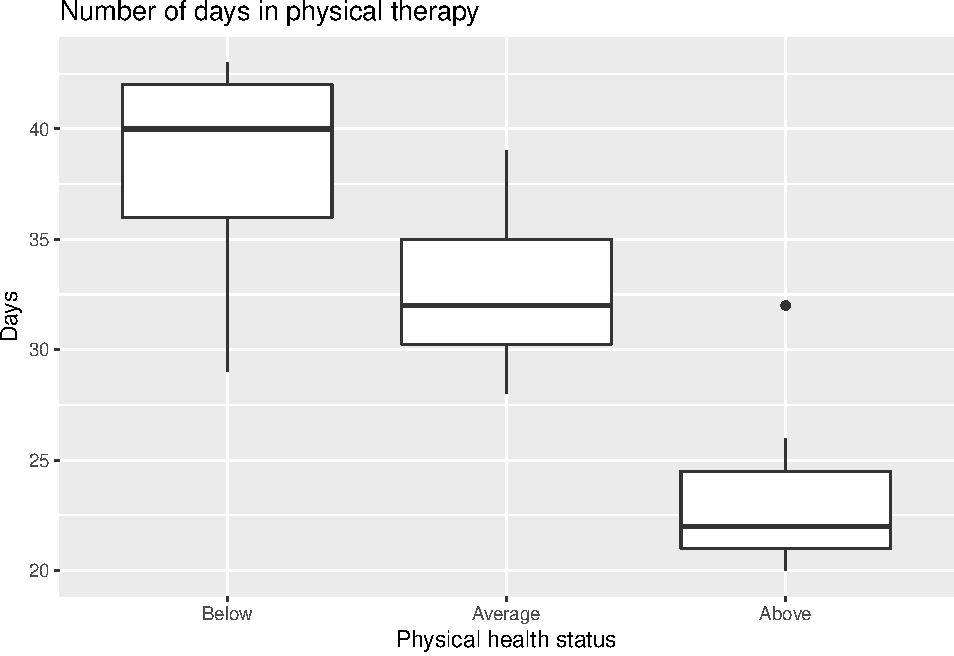
\includegraphics{hw3_files/figure-latex/unnamed-chunk-7-1.pdf}

\subsubsection{2. Using a type I error of 0.01, obtain the ANOVA table.
State the hypotheses, decision rule and
conclusion.}\label{using-a-type-i-error-of-0.01-obtain-the-anova-table.-state-the-hypotheses-decision-rule-and-conclusion.}

The hypotheses for the ANOVA test are:

\(H_0: \mu_{\text{below}} = \mu_{\text{average}} = \mu_{\text{above}}\).
In other words, physical status has no effect on the amount of physical
therapy needed for rehabilitation. (Duration of physical therapy is the
same in all physical status categories)
\(H_1: \text{not all } \mu \text{ equal.}\) Physical status has some
effect on the amount of physical therapy needed for rehabilitation.
(Duration of physical therapy is different in at least one physical
status category)

With a sample size of 25 participants (n), 3 groups (k), and
\(\alpha = 0.01\), we will reject the null hypothesis in favor of the
alternative if the computed \(F\) statistic \(F\) is greater than the
critical value
\(F_{k-1, n-k, 1-\alpha} = F_{3-1,25-3,1-0.01} = F_{2,22,0.99} =\)
5.7190219.

\begin{longtable}[]{@{}lrrrrr@{}}
\toprule
& Df & Sum Sq & Mean Sq & F value & Pr(\textgreater{}F)\tabularnewline
\midrule
\endhead
factor(physical\_status) & 2 & 795.2457 & 397.62286 & 19.2802 &
1.45e-05\tabularnewline
Residuals & 22 & 453.7143 & 20.62338 & NA & NA\tabularnewline
\bottomrule
\end{longtable}

As seen in the below ANOVA table, our F-statistic for the test is 19.28.
Since 19.28 \textgreater{} 5.7190219, we reject the null in favor of the
alternative that physical status affects the amount of physical therapy
needed for rehabilitation.

\subsubsection{\texorpdfstring{3. Based on your response in part 3,
perform pairwise comparisons with the appropriate adjustments
(Bonferroni, Tukey, and Dunnett -- `below average' as reference). Report
your findings and comment on the differences/similarities between these
three
methods.}{3. Based on your response in part 3, perform pairwise comparisons with the appropriate adjustments (Bonferroni, Tukey, and Dunnett -- below average as reference). Report your findings and comment on the differences/similarities between these three methods.}}\label{based-on-your-response-in-part-3-perform-pairwise-comparisons-with-the-appropriate-adjustments-bonferroni-tukey-and-dunnett-below-average-as-reference.-report-your-findings-and-comment-on-the-differencessimilarities-between-these-three-methods.}

\begin{Shaded}
\begin{Highlighting}[]
\CommentTok{# multiple testing adjustments}
\KeywordTok{pairwise.t.test}\NormalTok{(knee_data}\OperatorTok{$}\NormalTok{days, knee_data}\OperatorTok{$}\NormalTok{physical_status, }\DataTypeTok{p.adj =} \StringTok{'bonferroni'}\NormalTok{)}
\end{Highlighting}
\end{Shaded}

\begin{verbatim}
## 
##  Pairwise comparisons using t tests with pooled SD 
## 
## data:  knee_data$days and knee_data$physical_status 
## 
##         Below   Average
## Average 0.0898  -      
## Above   1.1e-05 0.0011 
## 
## P value adjustment method: bonferroni
\end{verbatim}

\begin{Shaded}
\begin{Highlighting}[]
\KeywordTok{TukeyHSD}\NormalTok{(}\KeywordTok{aov}\NormalTok{(days}\OperatorTok{~}\KeywordTok{factor}\NormalTok{(physical_status), }\DataTypeTok{data =}\NormalTok{ knee_data))}
\end{Highlighting}
\end{Shaded}

\begin{verbatim}
##   Tukey multiple comparisons of means
##     95% family-wise confidence level
## 
## Fit: aov(formula = days ~ factor(physical_status), data = knee_data)
## 
## $`factor(physical_status)`
##                     diff       lwr        upr     p adj
## Average-Below  -5.000000 -10.41130  0.4113011 0.0736833
## Above-Below   -14.428571 -20.33278 -8.5243579 0.0000102
## Above-Average  -9.428571 -15.05051 -3.8066356 0.0010053
\end{verbatim}

\begin{Shaded}
\begin{Highlighting}[]
\KeywordTok{summary}\NormalTok{(multcomp}\OperatorTok{::}\KeywordTok{glht}\NormalTok{(}\KeywordTok{aov}\NormalTok{(days}\OperatorTok{~}\KeywordTok{factor}\NormalTok{(physical_status), }\DataTypeTok{data =}\NormalTok{ knee_data),}
               \DataTypeTok{lincft =} \KeywordTok{mcp}\NormalTok{(}\DataTypeTok{method =} \StringTok{"Dunnett"}\NormalTok{)))}
\end{Highlighting}
\end{Shaded}

\begin{verbatim}
## 
##   Simultaneous Tests for General Linear Hypotheses
## 
## Fit: aov(formula = days ~ factor(physical_status), data = knee_data)
## 
## Linear Hypotheses:
##                                     Estimate Std. Error t value Pr(>|t|)
## (Intercept) == 0                      38.000      1.606  23.667   <0.001
## factor(physical_status)Average == 0   -5.000      2.154  -2.321   0.0681
## factor(physical_status)Above == 0    -14.429      2.350  -6.139   <0.001
##                                        
## (Intercept) == 0                    ***
## factor(physical_status)Average == 0 .  
## factor(physical_status)Above == 0   ***
## ---
## Signif. codes:  0 '***' 0.001 '**' 0.01 '*' 0.05 '.' 0.1 ' ' 1
## (Adjusted p values reported -- single-step method)
\end{verbatim}

All three pairwise comparison tests conclude that those in the `above
average' health category spend significantly less (at a 1\% significance
level) time in physical therapy than those of average or below average
health, who spend a comparable amount of time in physical therapy.
Though all three adjustments conclude the same thing, notice that
Bonferroni is the most conservative of the bunch, yielding the highest
p-values and making it hardest to reject the null that there is a
difference in means (in this case, time spent in physical therapy)
between health levels. In terms of conservativeness, it is followed by
Tukey, and finally Dunnett.

\subsubsection{4. Write a short paragraph summarizing your results as if
you were presenting to the rehabilitation center
director.}\label{write-a-short-paragraph-summarizing-your-results-as-if-you-were-presenting-to-the-rehabilitation-center-director.}

Using this data, we are interested in knowing whether someone's overall
physical health status (e.g.~below, at, or above average) impacts the
amount of time needed in physical therapy in order to fully recover.
Since we have three categories of physical fitness, we can use an ANOVA
test to understand whether at least one of these groups has a
significantly different distribution of physical therapy duration.
According to this test, and at a 5\% significant level, we conclude that
in fact physical fitness does have an impact on the duration of physical
therapy. Upon further examination, people in the `above average'
category spend a significantly less amount of time (number of days) in
physical therapy, whereas there was no difference in the amount of time
spent in physical therapy for those of average or below average health.
Statisical results are provided above, as well as a figure depicting the
distribution of physical therapy duration in each group.

\newpage  

\subsubsection{\texorpdfstring{Problem 4: For this problem you will use
the built-in R data called ``UCBAdmissions'' (library `datasets'), an
example of sex bias in admission practices. You are interested in
comparing the proportions of women vs men admitted at Berkeley (over all
departments).}{Problem 4: For this problem you will use the built-in R data called UCBAdmissions (library datasets), an example of sex bias in admission practices. You are interested in comparing the proportions of women vs men admitted at Berkeley (over all departments).}}\label{problem-4-for-this-problem-you-will-use-the-built-in-r-data-called-ucbadmissions-library-datasets-an-example-of-sex-bias-in-admission-practices.-you-are-interested-in-comparing-the-proportions-of-women-vs-men-admitted-at-berkeley-over-all-departments.}

\subsubsection{1. Provide point estimates and 95\% CIs for the overall
proportions of men and women admitted at Berkeley. Briefly comment on
the
values.}\label{provide-point-estimates-and-95-cis-for-the-overall-proportions-of-men-and-women-admitted-at-berkeley.-briefly-comment-on-the-values.}

The below table gives the observed proportion of acceptances for men and
women, where each proportion is calculated as
\(\hat{p} = \frac{\text{total number of acceptances}}{\text{total number of applications}}\).

\begin{longtable}[]{@{}lrr@{}}
\toprule
Gender & Acceptances & Proportion of total applications\tabularnewline
\midrule
\endhead
Female & 557 & 0.304\tabularnewline
Male & 1198 & 0.445\tabularnewline
\bottomrule
\end{longtable}

To compute a 95\% CI for the proportion estimate \(\hat{p}\) in each
group, we need to first establish that the the data follows a normal
distribution (\(np(1-p) \geq 5\)). This is clearly true for men
(\((n_m)(p_m)(1-p_m) = (2691)(0.445)(1-0.445) = 664.61 > 5\)) and women
(\((n_w)(p_w)(1-p_w) = (1835)(0.304)(1-0.304) = 388.26 > 5\)), and so we
can assume a normal distributions. Therefore, the 95\% for any one group
is given by

\[(\hat{p} - z_{0.975}\sqrt{\frac{\hat{p}(1-\hat{p})}{n}}, \hat{p} + z_{0.975}\sqrt{\frac{\hat{p}(1-\hat{p})}{n}})\]

For men, this is equal to
\[(0.445 - z_{0.975}\sqrt{\frac{0.445(1-0.445)}{2691}}, 0.445 + z_{0.975}\sqrt{\frac{0.445(1-0.445)}{2691}}) = (0.426, 0.464)\]
Thus we are 95\% confident that between 42.6\% and 46.4\% of male
applicants are admitted to UC Berkeley across departments.

For women, we have
\[(0.304 - z_{0.975}\sqrt{\frac{0.304(1-0.304)}{1835}}, 0.304 + z_{0.975}\sqrt{\frac{0.304(1-0.304)}{1835}}) = (0.283, 0.325)\]
And we are 95\% confident that between 28.3\% and 32.5\% of female
applicants are admitted.

\subsubsection{\texorpdfstring{2. Perform a hypothesis test to assess if
the two proportions in 1) are significantly different. Report the
results including the test statistic and p-value and an overall
conclusion of your findings. This part should contain both `hand' and R
calculations. For the latter, feel free to use built-in functions or to
create your
own.}{2. Perform a hypothesis test to assess if the two proportions in 1) are significantly different. Report the results including the test statistic and p-value and an overall conclusion of your findings. This part should contain both hand and R calculations. For the latter, feel free to use built-in functions or to create your own.}}\label{perform-a-hypothesis-test-to-assess-if-the-two-proportions-in-1-are-significantly-different.-report-the-results-including-the-test-statistic-and-p-value-and-an-overall-conclusion-of-your-findings.-this-part-should-contain-both-hand-and-r-calculations.-for-the-latter-feel-free-to-use-built-in-functions-or-to-create-your-own.}

Because we're dealing with proportions in two populations (male and
female), we can perform a two-sample test of proportions. Our null
hypothesis is that the proportions of accepted men and women across all
departments are the same, and our alternative hypothesis is that they
are different; \[H_0: p_{men} - p_{women} = 0\]
\[H_1: p_{men} - p_{women} \neq 0\]

We don't need to test for equality of variances here since we operate
under a normality assumption (via part 1 above), and can calculate the
test statistic directly using the formula
\[z = \frac{\hat{p}_1 - \hat{p}_2}{\sqrt{\hat{p}(1-\hat{p})(\frac{1}{n_1} + \frac{1}{n2})}}, \text{ where } \hat{p} = \frac{n_1p_1 + n_2p_2}{n_1 + n_2}\].

Using R we find that \(\hat{p} = 0.38\) and \(z = -9.55\). Our p-value
for the hypothesis test is \textless{}0.0001, and we can conclude that
there is a difference in the proportion of men and women who are
accepted to UC Berkeley across all departments. Below is a function I
wrote to perform the hypothesis test, with an option to include a
continuity correction.

\begin{Shaded}
\begin{Highlighting}[]
\CommentTok{# p1, p2 = the proportion observed in groups 1 and 2}
\CommentTok{# n1, n2 = sample sizes in groups 1 and 2}
\CommentTok{# sig.level = significance (alpha) level. Default to 0.05}
\CommentTok{# cont.correction = logical (T/F) for whether to apply a continuity correction. }
\CommentTok{#                   Default is FALSE.}
\NormalTok{prop.z.test =}\StringTok{ }\ControlFlowTok{function}\NormalTok{(p1, p2, n1, n2, }\DataTypeTok{sig.level =} \FloatTok{0.05}\NormalTok{, }\DataTypeTok{cont.correction =} \OtherTok{FALSE}\NormalTok{)\{}
\NormalTok{  p.hat =}\StringTok{ }\NormalTok{(n1}\OperatorTok{*}\NormalTok{p1 }\OperatorTok{+}\StringTok{ }\NormalTok{n2}\OperatorTok{*}\NormalTok{p2) }\OperatorTok{/}\StringTok{ }\NormalTok{(n1 }\OperatorTok{+}\StringTok{ }\NormalTok{n2)}
\NormalTok{  p.bar =}\StringTok{ }\NormalTok{p1 }\OperatorTok{-}\StringTok{ }\NormalTok{p2}
  
  \ControlFlowTok{if}\NormalTok{ (cont.correction }\OperatorTok{==}\StringTok{ }\NormalTok{F) \{}
\NormalTok{    z =}\StringTok{ }\NormalTok{p.bar }\OperatorTok{/}\StringTok{ }\KeywordTok{sqrt}\NormalTok{(p.hat}\OperatorTok{*}\NormalTok{(}\DecValTok{1} \OperatorTok{-}\StringTok{ }\NormalTok{p.hat)}\OperatorTok{*}\NormalTok{(}\DecValTok{1}\OperatorTok{/}\NormalTok{n1 }\OperatorTok{+}\StringTok{ }\DecValTok{1}\OperatorTok{/}\NormalTok{n2))}
\NormalTok{  \} }\ControlFlowTok{else}\NormalTok{ \{}
\NormalTok{    z =}\StringTok{ }\NormalTok{(p.bar }\OperatorTok{-}\StringTok{ }\NormalTok{(}\DecValTok{1}\OperatorTok{/}\NormalTok{(}\DecValTok{2}\OperatorTok{*}\NormalTok{n1) }\OperatorTok{+}\StringTok{ }\DecValTok{1}\OperatorTok{/}\NormalTok{(}\DecValTok{2}\OperatorTok{*}\NormalTok{n2))) }\OperatorTok{/}\StringTok{ }\KeywordTok{sqrt}\NormalTok{(p.hat}\OperatorTok{*}\NormalTok{(}\DecValTok{1} \OperatorTok{-}\StringTok{ }\NormalTok{p.hat)}\OperatorTok{*}\NormalTok{(}\DecValTok{1}\OperatorTok{/}\NormalTok{n1 }\OperatorTok{+}\StringTok{ }\DecValTok{1}\OperatorTok{/}\NormalTok{n2))}
\NormalTok{  \}}
  
\NormalTok{  pval =}\StringTok{ }\DecValTok{1} \OperatorTok{-}\StringTok{ }\KeywordTok{pnorm}\NormalTok{(}\KeywordTok{abs}\NormalTok{(z))}
  
  \KeywordTok{return}\NormalTok{(}\KeywordTok{list}\NormalTok{(}
    \DataTypeTok{z =}\NormalTok{ z,}
    \DataTypeTok{phat =}\NormalTok{ p.hat,}
    \DataTypeTok{p.val =}\NormalTok{ pval}
\NormalTok{  ))}
\NormalTok{\}}
\end{Highlighting}
\end{Shaded}


\end{document}
